\documentclass[12pt]{article}

\usepackage{graphicx}

\title{\bf{Paper reading for Voronoi Diagram in The Laguerre Geometry and its Applications}}
\date{}
\usepackage{CJK}
\begin{document}

\maketitle

\begin{CJK}{UTF8}{bkai}

\centerline{\bf 問題定義}

本問題想要在 {\it Laguerre geometry} 上求出 {\it Voronoi diagram}。\\

將一個三維空間的點~$(x,y,z)$~對應到歐氏平面上是一個半徑為~$|z|$~且圓心為~$(x,y)$~的圓,
而且此圓的旋轉方向是根據~$z$~的正負值,則稱為 {\it Laguerre geometry}。\\

在二維空間的一圓~$C_i=C_i(Q_i;r_i)$~,其中圓心為~$Q_i=(x_i,y_i)$~
,半徑為~$r_i$~。~$C_i$~和~$P=(x,y)$~之間的距離~$d_L(C_i,P)$~之定義如下:

\begin{equation}
d_L^2(C_i,P)=(x-x_i)^2+(y-y_i)^2-r_i^2
\end{equation}

因此,在 {\it Laguerre geometry} 上 $n$ 個圓 $C_i=C_i(Q_i;r_i)(Q_i=(x_i,y_i))$ 的 {\it Voronoi polygons} 的定義如下:

\begin{equation}
V(C_i)=\cap_i \{P \in R^2 | d_L^2(C_i,P) \leq d_L^2(C_j,P) \}
\end{equation}

求出所有的 {\it Voronoi polygons} ,就是我們要的 {\it Voronoi diagram}。\\


\centerline{\bf 方法說明}

%devide
假設一個 set $S={C_i(Q_i;r_i)|i=1,2,...,n}$,我們要把 $S$ 分成兩個 subsets $L$ 和 $R$。也就是說,
根據所有 $Q_i$ 的 $x$ 座標大小找出中位數 $m$,再來分成兩個 subsets 如下式子:

\[
L=\{Q_i| x_i < m \},~R=\{Q_i| x_i \geq m \}
\]

分好之後,$L$ 和 $R$ 各自畫出它們的 {\it Voronoi diagram} ,再把兩個 {\it Voronoi diagram} 合併起來。\\

%merge

合併兩個 {\it Voronoi diagram} 之前,需要先找出兩者之間的 {\it dividing line}。 Dividing line
 是由兩個 {\it rays} 和多個 {\it line segments} 組成,所以第一個問題是要如何找出那兩個 rays。\\

%how to find the two rays ( see Lemma 7, or Lemma 5  )

一開始先建出 $L$ 和 $R$ 的 {\it convex hulls},它們的 convex hulls 分別是 CH($L$) 和 CH($R$),
然後再建出 $L \cup R$ 的 convex hulls CH($L \cup R$)。
把 CH($L \cup R$) 和另外兩個 convex hulls 做比較,就會發現有新的兩個 line segments 連接著
 CH($L$) 和 CH($R$)。
之後就從那兩個 line segments 求出兩個 rays。\\

從新生的 line segments 的特性觀察,發現有特性稱為 {\it degenerate}。所謂的 degenerate ,
是指新的 convex hull edges 與相鄰的舊的 convex hull edges 都在同一線上,如下面 Figure 1 所示:\\

%Fig. 5.(i)

\begin{figure}
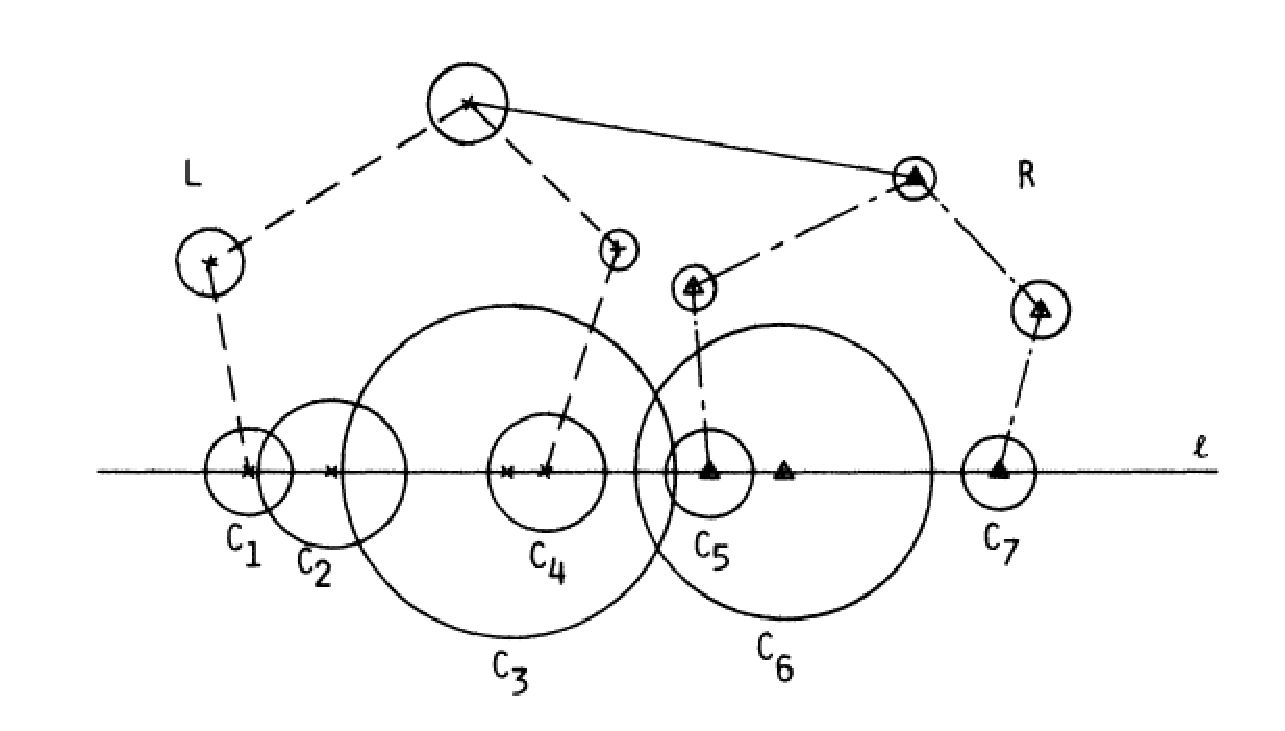
\includegraphics[scale=0.5]{figure5(i).eps}
\caption{}
\label{}
\end{figure}

明顯地,某些新舊 convex hull edges 都在 $l$ 線上。上圖 Figure 1 中上面實線部份,就是沒有 degenerate
 特性的例子。如果是沒有 degenerate 的特性,只要在 $l$ 上 $L$ 與 $R$ 中最接近的兩點取 {\it radical axis}
 即可;degenerate 的例子,則需要把 $l$ 分成 $L_l \subseteq L$ 和 $R_l \subseteq R$兩個集合。

%how to trace the several line segments ( see Lemma 4, and refer.[9]  )

從這兩條 rays 往圖形內部延伸,並且不斷地去做順時鐘方向和逆時鐘方向去調整,直到兩個 rays 連在一起,
就形成我們要的 dividing line。\\

\centerline{\bf 例子}

\centerline{\bf 時間複雜度分析}

\end{CJK}

\end{document}
